\section{8.31}
\paragraph{Specification:}
An isosceles triangle ABC, which is named in the mathematically positive direction, has the 
base AB with $A(-2|-1)$, $B(4|7)$ and the height h = 10E. 

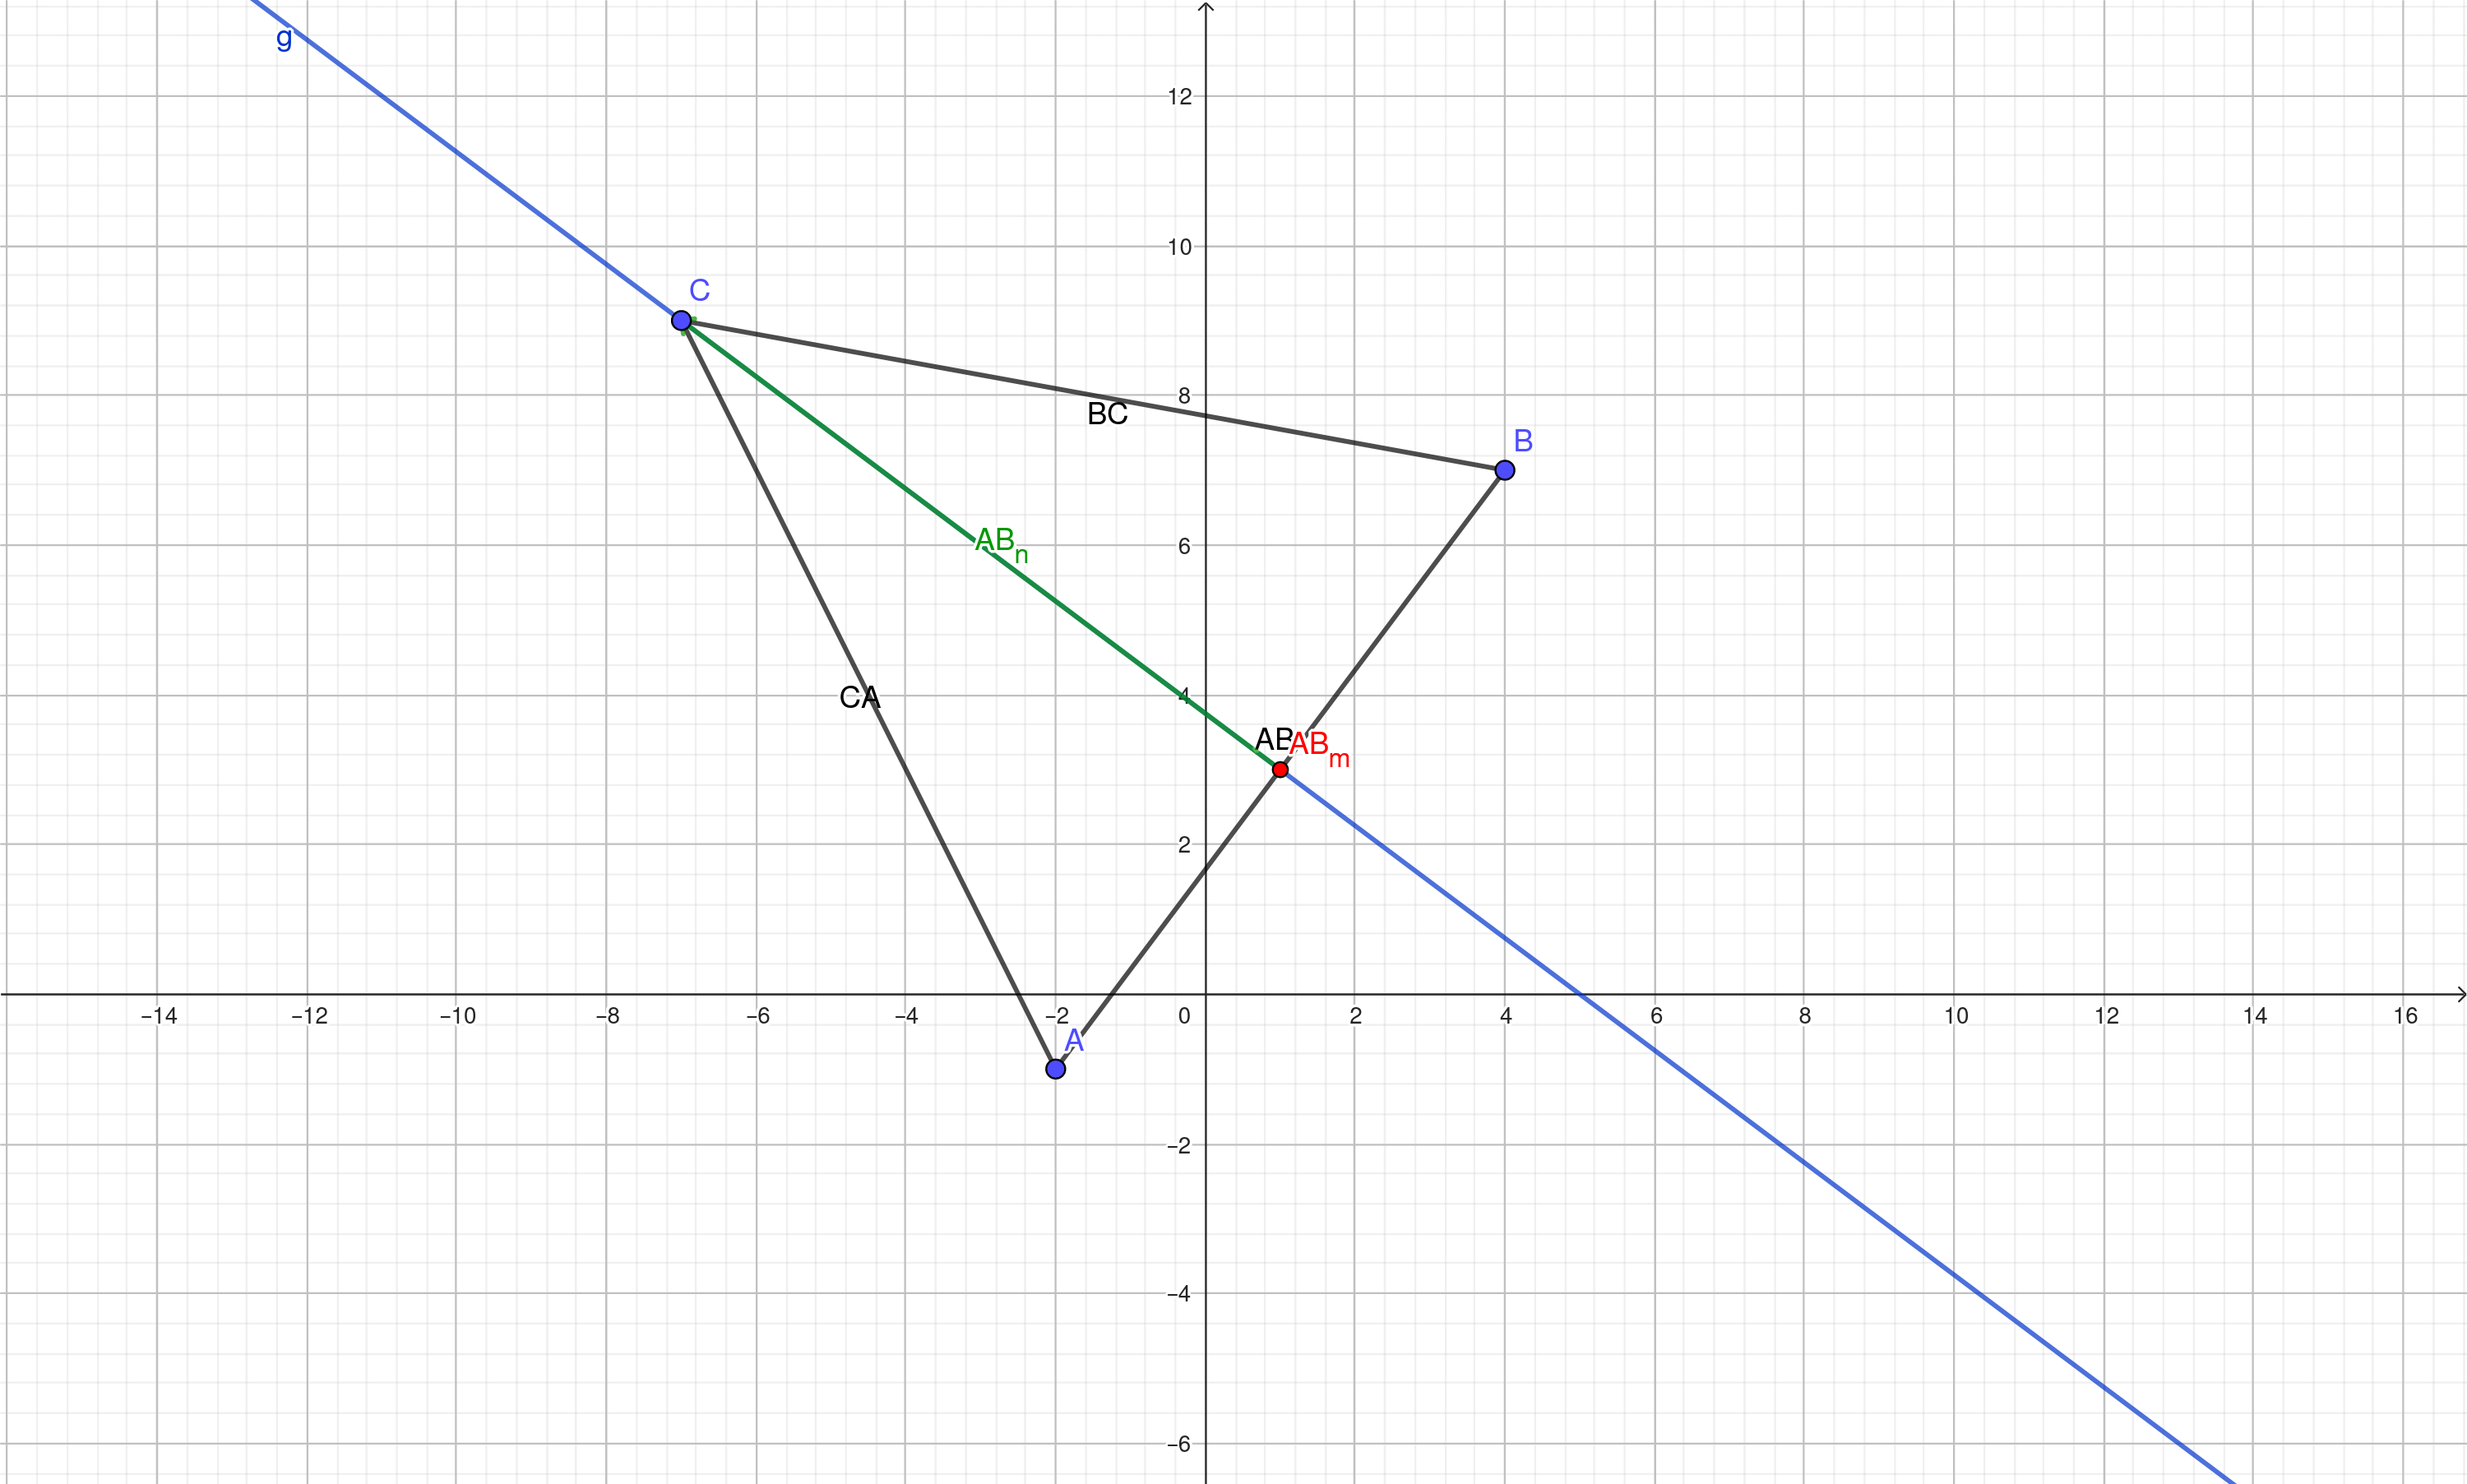
\includegraphics[width=\linewidth]{images/8-31.png}

\paragraph{Requirements:}
Calculate the missing point C, the angle $\phi$ which is enclosed by $\vec{AB}$ and $\vec{AC}$, 
and the area $A$ of the triangle.

\def\height{10}

\def\A{\begin{pmatrix}
    -2 \\ 
    -1
\end{pmatrix}}

\def\B{\begin{pmatrix}
    4 \\ 
    7
\end{pmatrix}}

\def\AB{\begin{pmatrix}
    6 \\ 
    8
\end{pmatrix}}

\def\vAC{\begin{pmatrix}
    -5 \\ 
    10
\end{pmatrix}}

\def\ABhalf{\begin{pmatrix}
    3 \\ 
    4
\end{pmatrix}}

\def\ABmid{\begin{pmatrix}
    1 \\ 
    3
\end{pmatrix}}

\def\ABnorm{\begin{pmatrix}
    -8 \\ 
    6
\end{pmatrix}}

\def\ABnrommag{\sqrt{(-8)^2 + 6^2}}

\def\ABmidzero{\begin{pmatrix}
    -0.8 \\ 
    0.6
\end{pmatrix}}

\def\vOC{\begin{pmatrix}
        -7 \\ 
        9
\end{pmatrix}}

\paragraph{Definitions:}
\begin{align}
    h &= \height E \\
    A &= \A \\
    B &= \B \\
    \vec{c} &= \vec{AB} \\
    \vec{c_m} &= \vec{OA} + \frac{1}{2} \vec{c}
\end{align}

\paragraph{Exercise:}
\subparagraph{Point $C$:}
\begin{align}
    \vec{c} &= \vec{OB} - \vec{OA} \\
    \vec{c} &= \B - \A \\
    \vec{c} &= \AB \\[20pt]
    \vec{c_m} &= \A + \frac{1}{2}\AB \\
    \vec{c_m} &= \A  + \ABhalf \\
    \vec{c_m} &= \ABmid \\[20pt]
    \vec{c_n} &= \ABnorm \\
    \vec{c_{n0}} &= \frac{1}{|\vec{c_n}|}\vec{c_n} \\
    \vec{c_{n0}} &= \frac{1}{\ABnrommag}\ABnorm \\
    \vec{c_{n0}} &= \frac{1}{10}\ABnorm \\
    \vec{c_{n0}} &= \ABmidzero \\[20pt]
    \vec{OC} &= \ABmid + \height\ABmidzero \\
    \vec{OC} &= \vOC
\end{align}

\subparagraph{Angle $\phi$:}
\begin{align}
    \vec{AC} &= \vec{OC} - \vec{OA} \\
    \vec{AC} &= \vOC - \A \\
    \vec{AC} &= \vAC \\[20pt]
    \cos(\phi) &= \frac{\vec{AB} \cdot \vec{AC}}{|\vec{AB}| * |\vec{AC}|} \\
    \cos(\phi) &= \frac{\AB \cdot \vAC}{\sqrt{6^2 + 8^2} * \sqrt{(-5)^2 + 10^2}} \\
    \cos(\phi) &= \frac{50}{111.803398875} \\
    \phi &= \arccos(0.4472135955) \\
    \phi &= 63.43495^\circ
\end{align}

\subparagraph{Area:}
\begin{align}
    A &= \frac{1}{2}ch_c \\
    A &= 5c \\[20pt]
    c &= |\vec{c}| \\
    c &= \sqrt{6^2 + 8^2} \\
    c &= 10 \\[20pt]
    A &= 50E^2
\end{align}

\paragraph{Answer:}
The point $C$ is at the location $(-7|9)$, the angle between $\vec{AB}$ and $\vec{AC}$ is 
$63.43495^\circ$, and the area of the triangle is 50$E^2$. 
